\newpage
\section{Suggested solutions: Time-frequency Uncertainty Principle}

\begin{enumerate}
\item The Hann window in continuous-time is defined as:
$$h_{1}(t)=\begin{cases}
    \sin^{2}(\pi t/T), \quad 0\le t\le T, \\
    0, \quad \text{otherwise}.
\end{cases}$$
Define the length of the Hann filter to be $T$ in time-domain. The Fourier transform of $h_{1}(t)$ can be shown to be
$$\mathcal{H}_{1}(\omega)=\left[\frac{\sin(\frac{T}{2}\omega)}{\omega}+\frac{1}{2}\frac{\sin(\pi-\frac{T}{2}\omega)}{\frac{2\pi}{T}-\omega}+\frac{1}{2}\frac{\sin(\pi+\frac{T}{2}\omega)}{\frac{2\pi}{T}+\omega}\right]e^{-i\frac{T}{2}\omega}.$$
Let $h_{2}(t)$ denote the rectangular window of length $T$, for which the Fourier transform is:
$$\mathcal{H}_{2}(\omega)=\frac{2\sin(\frac{T}{2}\omega)}{\omega}e^{-i\frac{T}{2}\omega},$$
which also has length taken to be $T$. 

\begin{enumerate}[a)]
\item Using the Fourier transform we have:
\begin{align*}
    \mathcal{H}_{1}(\omega)&=\int_{-\infty}^{\infty}\sin^{2}(\pi t/T)e^{-i\omega t}dt=\frac{1}{(2i)^{2}}\int_{0}^{T}\left(e^{i \pi t/T}-e^{-i\pi t/T}\right)^{2}e^{-i\omega t}dt, \\
    &=-\frac{1}{4}\int_{0}^{T}\left[e^{-i(\omega -2\pi/T)t}-2e^{-i\omega t}+e^{-i(\omega + 2\pi/T)t}\right]dt. \\
\end{align*}
Last handle each term on its own, the first term is computed as 
\begin{align*}
    \int_{0}^{T}e^{-i(\omega-2\pi/T)t}dt&=\left[-\frac{1}{i(\omega-\frac{2\pi}{T})}e^{-i(\omega-2\pi/T)t}\right]_{0}^{T}=\frac{1}{i(\omega-\frac{2\pi}{T})}(1-e^{-i(\omega T-2\pi)}), \\
    &=\frac{1}{i(\omega-\frac{2\pi}{T})}(e^{i(\omega T/2-\pi)}-e^{-i(\omega T/2-\pi)})e^{-i(\omega T/2-\pi)}, \\
    &=\frac{2}{\omega-\frac{2\pi}{T}}\sin\left(\omega\frac{T}{2}-\pi\right)e^{-i\omega\frac{T}{2}}\overbrace{e^{i\pi}}^{-1}, \\
    &=-\frac{2}{\frac{2\pi}{T}-\omega}\sin\left(-\left(\pi-\omega\frac{T}{2}\right)\right)e^{-i\omega\frac{T}{2}}(-1), \\
    &=-\frac{2}{\frac{2\pi}{T}-\omega}\sin\left(\pi-\omega\frac{T}{2}\right)e^{-i\omega\frac{T}{2}}
\end{align*}
the last step uses $\sin(-\theta)=-\sin(\theta)$. The second term is:
\begin{align*}
    \int_{0}^{T}e^{-i\omega t}dt&=\left[-\frac{1}{i\omega}e^{-i\omega t}\right]_{0}^{T}=\frac{1}{i\omega}(1-e^{-i\omega T}) \\
    &=\frac{1}{i\omega}(e^{i\omega T/2}-e^{-i\omega T/2})e^{-i\omega T/2}=\frac{2}{\omega}\sin\left(\omega\frac{T }{2}\right)e^{-i\omega\frac{T}{2}}
\end{align*}
and finally, the same approach as the first 
\begin{align*}
    \int_{0}^{T}e^{-i(\omega+2\pi/T)t}dt&=\left[-\frac{1}{i(\omega+\frac{2\pi}{T})}e^{-i(\omega+2\pi/T)t}\right]_{0}^{T}=\frac{1}{i(\omega+\frac{2\pi}{T})}(1-e^{-i(\omega T + 2\pi)}), \\
    &=\frac{1}{i(\omega+\frac{2\pi}{T})}(e^{i(\omega T/2+\pi)}-e^{-i(\omega T/2+\pi)})e^{-i(\omega T/2+\pi)}, \\
    &=\frac{2}{\omega+\frac{2\pi}{T}}\sin\left(\omega\frac{T}{2}+\pi\right)e^{-i\omega\frac{T}{2}}\overbrace{e^{-i\pi}}^{-1}, \\
    &=-\frac{2}{\frac{2\pi}{T}+\omega}\sin\left(\pi+\omega\frac{T}{2}\right)e^{-i\omega\frac{T}{2}}.
\end{align*}
Putting everything together with the correct signs and factors we obtain:
$$\mathcal{H}_{1}(\omega)=\left[\frac{\sin\left(\omega\frac{T }{2}\right)}{\omega}+\frac{1}{2}\frac{\sin\left(\pi-\omega\frac{T}{2}\right)}{\frac{2\pi}{T}-\omega}+\frac{1}{2}\frac{\sin\left(\pi+\omega\frac{T}{2}\right)}{\frac{2\pi}{T}+\omega}\right]e^{-i\frac{T}{2}\omega}$$
as desired.

\item If the peak of the Hann window is at $t=T/2$, then we can shift the peak to be at $t=0$ as follows
$$h(t)=h_{1}\left(t-\frac{T}{2}\right)=\sin^{2}\left(\frac{\pi}{T}\left(t-\frac{T}{2}\right)\right)=\sin^{2}\left(\frac{\pi}{T}t-\frac{\pi}{2}\right)=\cos^{2}\left(\frac{\pi}{T}t\right)$$
as $\sin\left(\theta-\frac{\pi}{2}\right)=-\cos(\theta)$. 

\item To plot the spectral responses, we can use Listing \ref{code14_1}.
\begin{lstlisting}[language=Python, caption=Filter spectral response,label=code14_1]
import numpy as n
import matplotlib.pyplot as plt

# frequency response for the Hann window with T = 1
def H1(omega):
    return (n.sin(omega/2)/omega + (1/2)*n.sin(n.pi - (1/2)*omega)/(2*n.pi - omega) + (1/2)*n.sin(n.pi + (1/2)*omega)/(2*n.pi + omega))*n.exp(-1j*1/2*omega)

# frequency response for the rectangular window with T = 1
def H2(omega):
    return 2*n.sin(omega/2)/omega*n.exp(-1j*1/2*omega)

# function to convert to dB
def convert_to_decibel(x):
    return 10*n.log10(n.abs(x)**2)

# partition the interval (-10pi,10pi) into 1000 equally spaced points
x = n.linspace(-10*n.pi,10*n.pi,num=1000)

# plot the window functions to compare 
# radians per sample on the x-axis and dB on the y-axis
plt.plot(x,convert_to_decibel(H1(x)),label="Hann window")
plt.plot(x,convert_to_decibel(H2(x)),label="Rectangular window")
plt.xlabel("$\hat{\omega}$")
plt.ylim(-120,10)   # limit the y-axis to (-120,10)
plt.legend()
plt.show()
\end{lstlisting}
The magnitude response is shown in Figure \ref{ex:filters}. The Figure shows that the Hann window manages the rejection of frequencies out of the band-pass better than the rectangular window. 
\begin{marginfigure}
    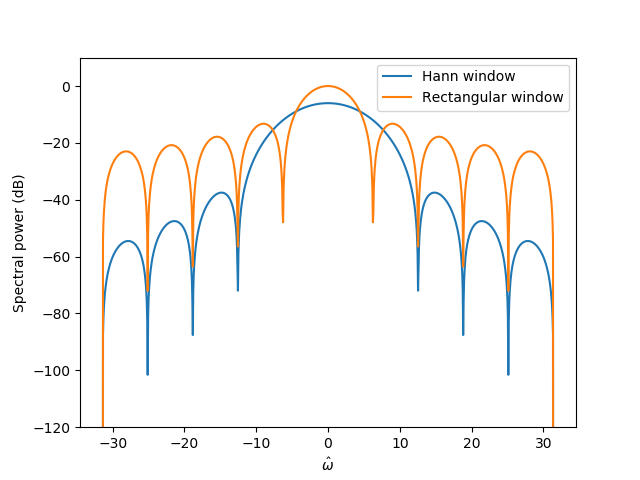
\includegraphics[width=7.0cm,height=7.5cm]{ch14/figures/filters.png}
    \caption{Comparison of the spectral responses of two filters}
    \label{ex:filters}
\end{marginfigure}

\item By inspecting Figure \ref{fig:hann_ct_ex_mr} we conclude that the rectangular window (in red) has its first zero at $\omega=\omega_{2}$, while the Hann window (in blue) has the first zero at $\omega=\omega_{1}$. By investigating the plot it appears that $\omega_{1}=2\omega_{2}$, where $\omega_{2}=2\pi /T$ as given. The width of the rectangular window is then $\Delta\omega_{2}=2\omega_{2}=4\pi/T$, meaning that the width of the Hann window is $\Delta\omega_{1}=2\omega_{1}=2(4\pi/T)=2\Delta\omega_{2}=8\pi /T$. 

\item We've shown that 
\begin{align*}
    \Delta\omega_{1}&=4\pi/T, \\
    \Delta\omega_{2}&=8\pi/T,
\end{align*}
so the rectangular window needs to be $T=2$ seconds long, while the Hann window needs to be $T=4$ seconds long. 

\item By Figure \ref{fig:hann_ct_ex_mr}: the Hann window cuts the power to approximately $-60\ \text{dB}$, which is around $10^{-6}$, while the rectangular window only cuts around $-20\ \text{dB}$ which corresponds to $10^{-2}$, so not that much reduction. The Hann window does a far better job in reducing the edges than the rectangular window.

\item As discussed in f) the Hann window is much better at handling frequencies outside the band-pass. This can be seen from the plot of the power of the magnitude response. Thus, the Hann window can be used much more efficiently to reduce spectral leakage which in many cases can be a huge problem, so the trade-off when comparing filter width to spectral leakage, reducing the leakage is preferred over reducing the filter width.


\end{enumerate}
\end{enumerate}